% Adapted from Gelugor theme example by:
% LIM Lian Tze <liantze@gmail.com>, 2011
% http://liantze.penguinattack.org/latextypesetting

\documentclass{beamer}
\usetheme{UB}
\usepackage{wrapfig}
\usepackage{amsmath}
\usepackage{amsfonts}
\usepackage{graphicx}
\graphicspath{{./figures}{./figures/factorgraph}}

%% Use any fonts you like.
%\usepackage{helvet}

\title{Occupancy grids and Dual Decomposition}
%\subtitle{A subtitle}
\author{Vikas Dhiman}
\date{\today}
\institute{\url{vikasdhi@buffalo.edu}}

% Adjust your address/title page text with the \address command
\renewcommand{\address}
{
	Vision and Perceptual Machines Lab\\
}

%% Uncomment to change the pic on the title frame
%% Sizing and placement currently only look good with landscape orientation, not portrait
%\renewcommand{\titlepic}{some_other_title_frame_image}

\begin{document}

\begin{frame}
\titlepage
\end{frame}


\section{Introduction}

\begin{frame}
\frametitle{Occupancy Grid to factor graph}
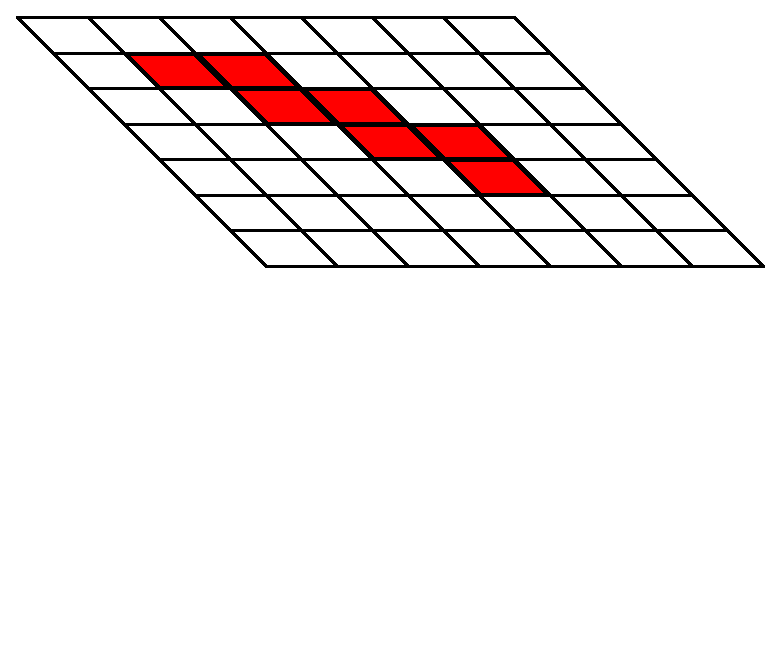
\includegraphics[width=\textwidth]{figures/factorgraph/fg0.pdf}
\end{frame}

\begin{frame}
\frametitle{Occupancy Grid to factor graph}
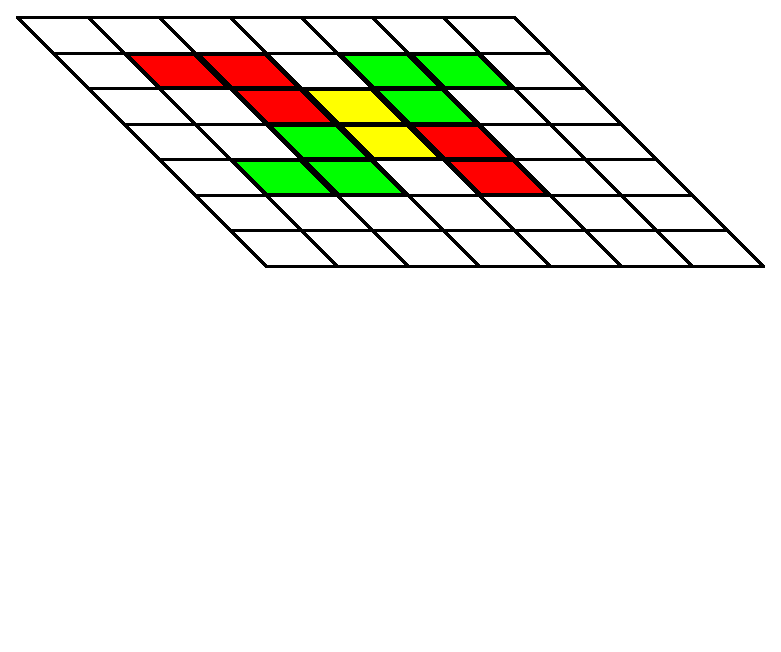
\includegraphics[width=\textwidth]{figures/factorgraph/fg1.pdf}
\end{frame}

\begin{frame}
\frametitle{Occupancy Grid to factor graph}
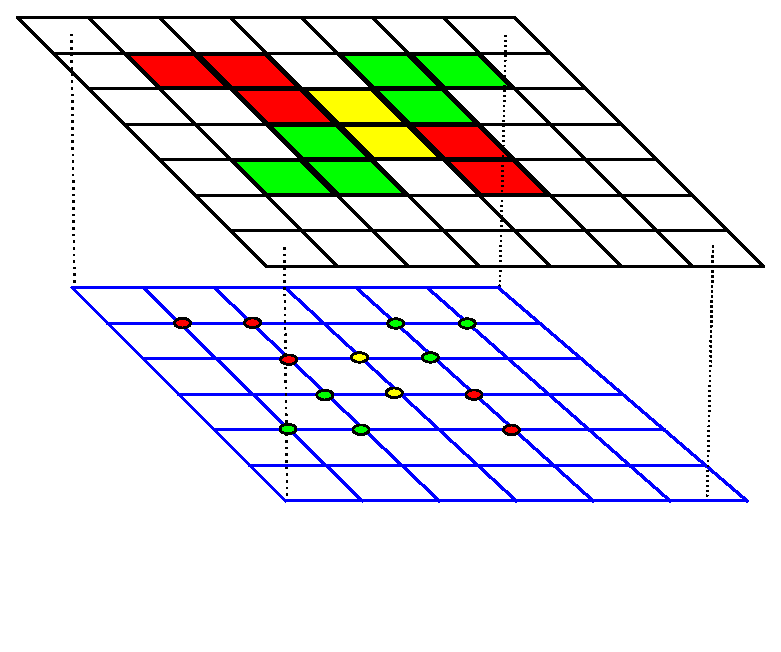
\includegraphics[width=\textwidth]{figures/factorgraph/fg2.pdf}
\end{frame}

\begin{frame}
\frametitle{Occupancy Grid to factor graph}
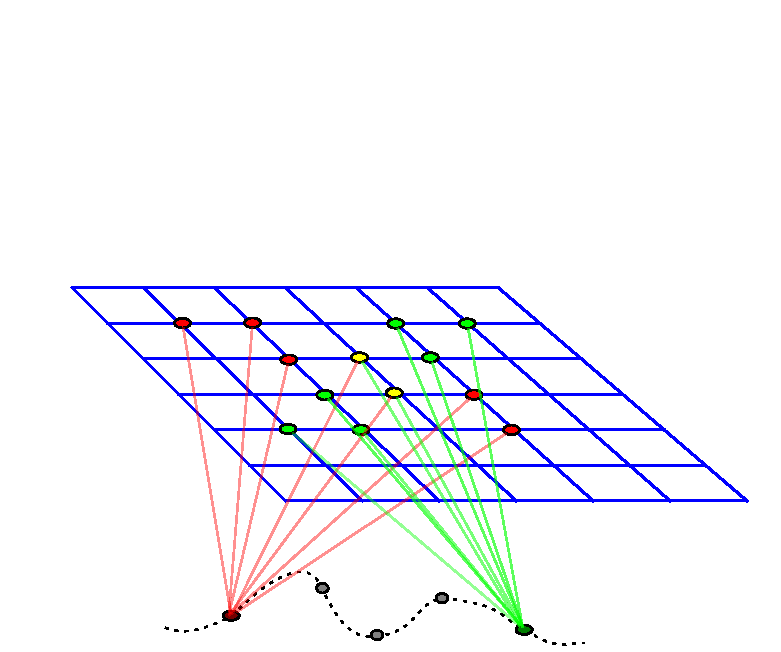
\includegraphics[trim=0in 0in 0in 2in, width=\textwidth]{figures/factorgraph/fg3.pdf}
\end{frame}

\begin{frame}
\frametitle{Notation}
\begin{columns}
  \begin{column}{0.7\textwidth}
    \begin{itemize}
      \item $m^r_k$ = Occupancy of $k^{th}$ cell of $r^{th}$ revision of map $m$
      \item $x_t$ = Pose (position + angle) of $t^{th}$ laser observation
      \item $z_t$ = Range observation given by $t^{th}$ laser observation
      \item $f_t = f(m, x_t)$\\
        = First occupied cell in map $m$ that blocks laser for $t^{th}$ observation
    \end{itemize}
  \end{column}
  \begin{column}{0.3\textwidth}
    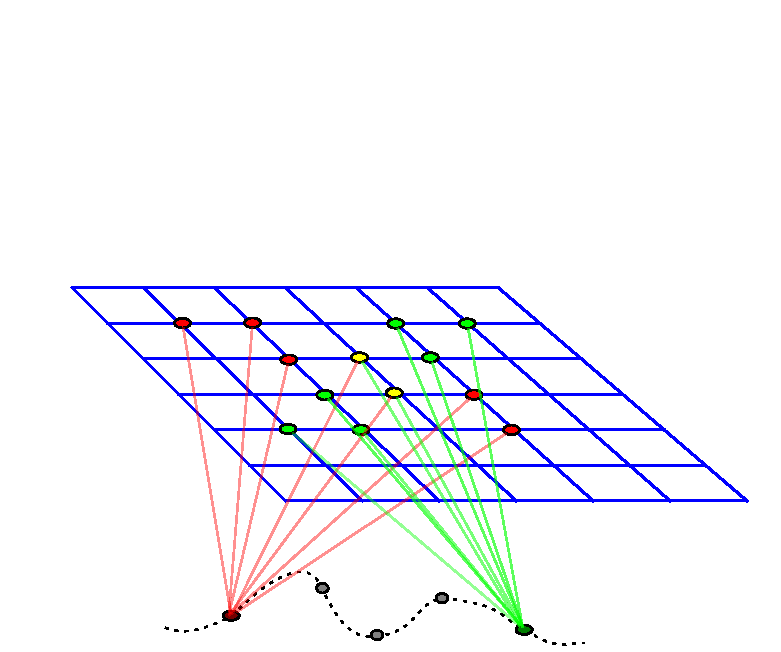
\includegraphics[trim=0in 0in 0in 2in, width=\textwidth]{figures/factorgraph/fg3.pdf}
  \end{column}
\end{columns}
\end{frame}
\begin{frame}
  \frametitle{Full solution}
  \begin{figure}
    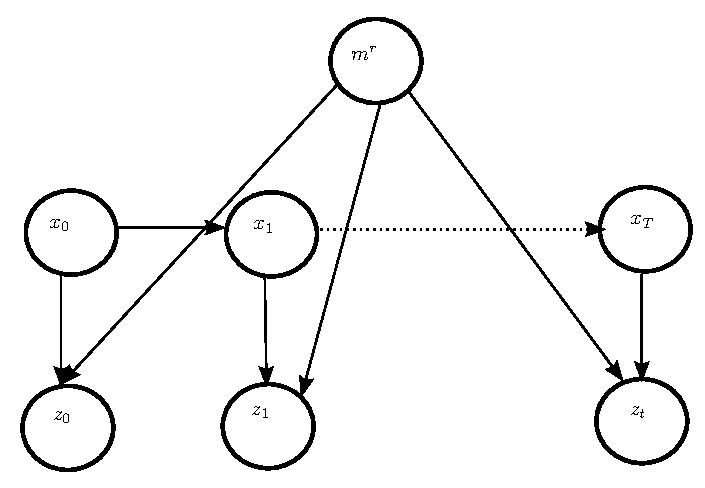
\includegraphics[width=0.3\textwidth]{figures/mrf_model_wrapper.pdf}
  \end{figure}
  \begin{align}
    p(m^r|z, x) &= \frac{1}{Z} p(z_T|m^r, z_{1:t-1}, x)p(m^r|z_{1:t-1},x)\\
                &= \frac{1}{Z} p(z_T|m^r, x_T)p(m^r|z_{1:t-1}, x_{1:t-1})\\
                &= \frac{1}{Z} p(z_T|f^r_T)p(m^r|z_{1:t-1}, x_{1:t-1})\\
                %&= \frac{1}{Z} p(m^r)\prod_{t=1}^{T}p(z_t|f^r_t)\\
    p(m_k|z, x) &= \sum_{r}p(m_k|m_r)p(m^r|z, x)
  \end{align}
\end{frame}
\begin{frame}
  \frametitle{Two assumption method}
  \begin{figure}
    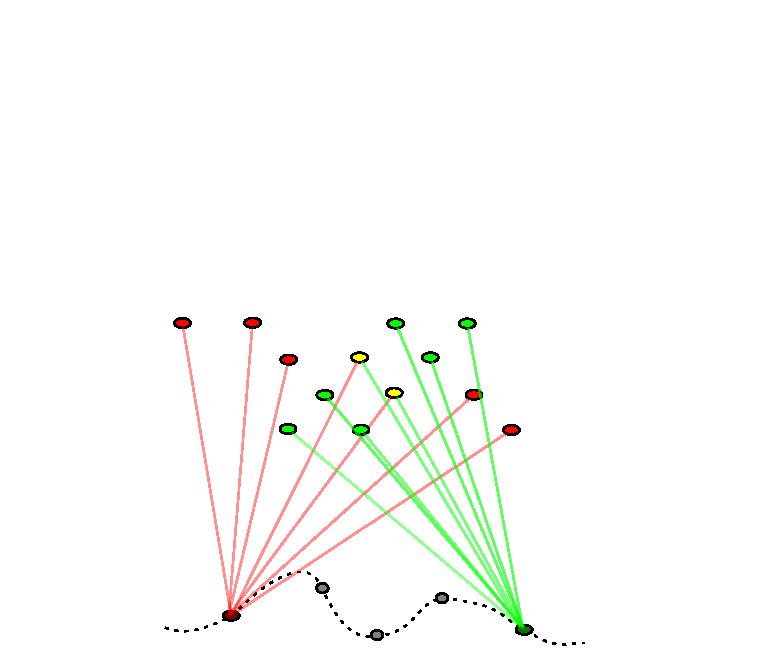
\includegraphics[trim=0in 0in 0in 2in, width=0.3\textwidth]{figures/factorgraph/fg_two_assumption.pdf}
  \end{figure}
  Assumptions:
  \begin{align}
    p(m) &= \prod p(m_k)\\
p(z|m_k) &= \prod p(z_t|m_k)
  \end{align}
  Simplified equations:
  \begin{align}
    p(m_k|z, x) &= \frac{1}{Z} p(z_T|m_k, z_{1:t-1}, x)p(m|z_{1:t-1},x)\\
                &= \frac{1}{Z} p(z_T|m_k, x_T)p(m|z_{1:t-1},x)\\
                &= \frac{1}{Z} p(m_k|z_T, x_T)p(z_T|x_T)p(m|z_{1:t-1},x)
  \end{align}
\end{frame}
\begin{frame}
  \frametitle{Gibbs sampling (Merali2013icra)}
  For Gibbs sampling we need conditional probability.
  \begin{align}
    p(m_k|\mathbf{z},\mathbf{x}, m_{\neg k}) &= p(m_k|m_{\neg k})\prod_{t=0}^{T}p(z_t|m, x_t)\\
                               p(z_t|m, x_t) &= N(z_t|\text{pos($f_t$)}, d^2)\\
                                           d &= \text{distance between $z_t$ and $f_t$}
  \end{align}
\end{frame}
\begin{frame}
  \frametitle{Notation}
  \begin{itemize}
      \item $\kappa_t = \kappa(z_t, x_t)$ = $[\kappa^i_t]_{i=1}^{n}$ \\
        = List of $n$ cells that laser goes through for $t^{th}$ observation when travels for $z_t$ units.
  \end{itemize}
  \begin{figure}
    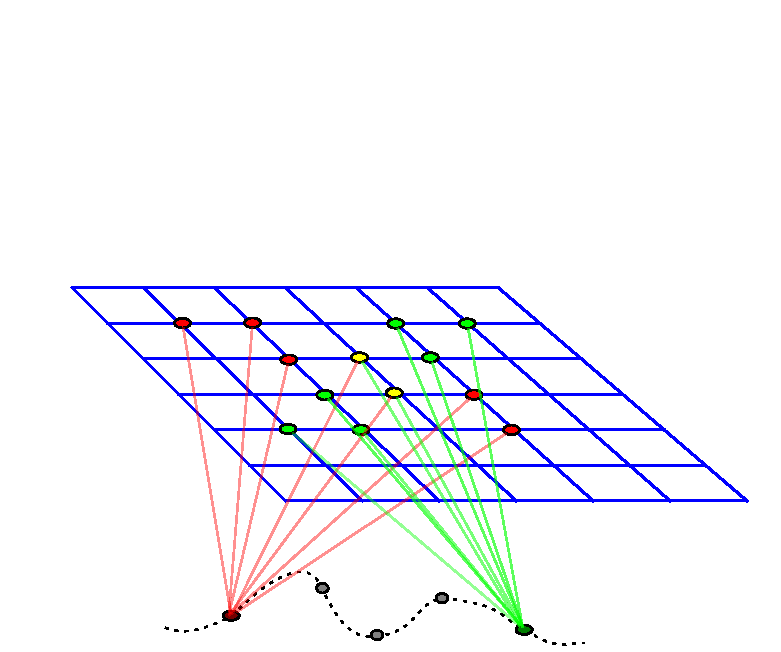
\includegraphics[trim=0in 0in 0in 2in, width=0.7\textwidth]{figures/factorgraph/fg3.pdf}
  \end{figure}
\end{frame}
\begin{frame}
  \frametitle{Factorization (Brian's technique)}
  \begin{align}
    p(m_k|z, x, m_{neg k}) &= \frac{1}{Z} p(m_k|m_{\neg k}) \prod_t p(z_t|m, x_t)\\
                           &= \frac{1}{Z} p(m_k|m_{\neg k}) \prod_t p(z_t|m_{\kappa_t}, x_t)\\
  p(z_t|m_{\kappa_t}, x_t) &= \frac{1}{Z'}exp(-E(m_{\kappa_t}, z_t, x_t))\\
  E(m_{\kappa_t}, z_t, x_t) &= \begin{cases}
              0 & \text{if $m_{k} = 0 \forall k \in \{\kappa^i_t\}_{i=1}^{n-1} \land m_{\kappa_t^n} = 1$}\\
            900 & \text{if $m_{k} = 0 \forall k \in \{\kappa^i_t\}_{i=1}^{n-1} \land m_{\kappa_t^n} = 0$}\\
           1000 & \text{ otherwise}
    \end{cases}
  \end{align}

\end{frame}
\begin{frame}
  \begin{figure}
    
\includegraphics[width=0.3\textwidth]{figures/gt-final.png}
    
\includegraphics[width=0.3\textwidth]{figures/mcmc_100x100.png}
    
\includegraphics[width=0.3\textwidth]{figures/two-assumption_100x100.png}
    \caption{From left to right: 1) Observed ground truth (resolution: 500x500) 2) Gibbs sampling merali2013icra $20 \times 10^4$ samples(resolution:100x100) 3) Two-assumption method (resolution:500x500) }
    \label{fig:results}
  \end{figure}
\end{frame}

\begin{frame}
  With occupancy prior 0.5
  \begin{figure}
    
\includegraphics[width=0.3\textwidth]{figures/Metropolis_Marginals_20k_iter.png}
    
\includegraphics[width=0.3\textwidth]{figures/Metropolis_Marginals_40k_iter.png}
    
\includegraphics[width=0.3\textwidth]{figures/metropolis_100x100.png}
    \caption{From left to right: Marginals computed by metropolis hastings algorithm with 1) $2 \times 10^4$ samples (resolution:100x100) 2) with $4 \times 10^4$ samples and 3) with $10 \times 10^4$ samples }
    \label{fig:metropolis-results}
  \end{figure}
\end{frame}

\begin{frame}
  With occupancy prior 0.3
  \begin{figure}
    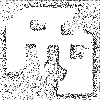
\includegraphics[width=0.3\textwidth]{figures/occgridvis200.png}
    
\includegraphics[width=0.3\textwidth]{figures/occgridvis400.png}
    
\includegraphics[width=0.3\textwidth]{figures/occgridvis600.png}
    \caption{From left to right: Marginals computed by metropolis hastings algorithm with 1) $2 \times 10^4$ samples (resolution:100x100) 2) with $4 \times 10^4$ samples and 3) with $6 \times 10^4$ samples }
    \label{fig:metropolis-results}
  \end{figure}
\end{frame}

\begin{frame}
  With occupancy prior 0.3 and resolution 200x200.
  \begin{figure}
    
\includegraphics[width=0.3\textwidth]{figures/occgridvis200_200x200.png}
    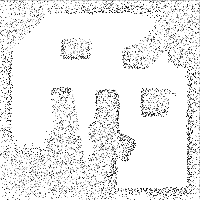
\includegraphics[width=0.3\textwidth]{figures/occgridvis400_200x200.png}
    
\includegraphics[width=0.3\textwidth]{figures/occgridvis600_200x200.png}
    \caption{From left to right: Marginals computed by metropolis hastings algorithm with 1) $2 \times 10^4$ samples (resolution:100x100) 2) with $4 \times 10^4$ samples and 3) with $6 \times 10^4$ samples }
    \label{fig:metropolis-results}
  \end{figure}
\end{frame}

\end{document}
